

\chapter{Domain Shift Anatomy}
%\chapter{Domain shift in MR images}
\label{chap:mri}


% The inherent differences in image acquisition protocols can lead to significant performance degradation in convolutional neural networks (CNNs) when applied to unseen domains.
This chapter addresses the challenge of supervised domain adaptation in medical image segmentation, with a specific focus on the variability in MRI scans across different clinical sites. Firstly, we investigate that fine-tuning the initial layers of a convolutional neural network (CNN), which are more sensitive to low-level image features such as intensity variations, can more effectively mitigate domain shifts and enhance segmentation accuracy, particularly under conditions where annotated data is scarce. Then, we introduce SpotTUnet, a novel CNN architecture designed to autonomously determine the optimal layers for fine-tuning based on the characteristics of the target domain. SpotTUnet not only achieves competitive segmentation accuracy but also provides insights into which layers are most susceptible to domain shifts. Collectively, these two studies are invaluable for understanding the underlying dynamics of domain adaptation in medical image segmentation and can guide future research and practical implementations.
%improving the reliability of medical image segmentation across diverse clinical environments.


\section{Introduction}

Convolutional Neural Networks (CNNs) have emerged as the most accurate methods for segmentation in many medical image analysis tasks \cite{shen2017deep}. The key strength of deep CNNs is their remarkable flexibility, enabled by a vast number of trainable parameters. However, this flexibility can also lead to significant performance degradation when the test data differs in distribution from the training data, a frequent issue in medical imaging \cite{wang2018deep}. This challenge is particularly pronounced in Magnetic Resonance Imaging (MRI), where variations in scanning protocols can result in differences in slice orientation, thickness, and, most critically, overall image intensities \cite{kamnitsas2017unsupervised,glocker2019machine,orbes2019multi}. Such differences between training and testing domains, commonly referred to as \textit{domain shift}, necessitate the use of Domain Adaptation (DA) methods.

Many existing DA approaches focus on fine-tuning the later layers of CNNs, operating under the assumption that low-level features are shared across domains and tasks, while high-level features are more susceptible to changes and thus require adaptation \cite{yosinski2014transferable}. However, we hypothesize that the variations in MRI intensities are mostly low-level, which are primarily captured by the early convolutional layers, and can be effectively addressed by fine-tuning these initial layers. Through a comparative analysis of several fine-tuning strategies---including fine-tuning the entire network, the initial layers, and the final layers---we demonstrate that fine-tuning the initial layers significantly outperforms fine-tuning the final layers. Furthermore, in scenarios with extremely limited annotated data, fine-tuning the initial layers appears to be more effective than fine-tuning the entire network.

Nonetheless, the question of finding the optimal fine-tuning strategy remains, since we tested only a limited number of options. Here, we adopt SpotTune \cite{guo2019spottune}, a Transfer Learning (TL) approach, that offers an adaptive fine-tuning mechanism by learning a policy that determines which layers should be either fine-tuned or re-used. We extend the SpotTune approach to the DA problem in medical image segmentation, proposing a novel method called SpotTUnet. Moreover, we suggest an interpretation mechanism to indicate CNN layers that are most susceptible to domain shift, providing insights into the nature of MRI domain shifts. Thus, SpotTUnet not only improves the supervised DA results but also provides the interpretable visualization, \textit{domain shift anatomy}, which could be used to enhance the unsupervised DA methods.\\

%\let\labelitemi\labelitemii
%\noindent
Our contribution in this chapter is threefold:
\begin{enumerate}
	\item \textbf{Predefined fine-tuning.} We show that fine-tuning the initial layers of a CNN significantly outperforms fine-tuning the final layers, and, under conditions of extremely limited data, it also outperforms fine-tuning the entire network.
	\item \textbf{Adaptive fine-tuning.} We introduce SpotTUnet, the first adaptation of SpotTune \cite{guo2019spottune} for supervised DA in medical image segmentation. SpotTUnet performs on par with the best alternative fine-tuning methods across different data availability scenarios.
	\item \textbf{Domain shift anatomy.} We provide a detailed analysis of optimal fine-tuning strategies across various data availability scenarios, offering insights into the underlying reasons for the observed performance differences.
\end{enumerate}
% , incorporating interpretable regularization


\section{Related work}

The most common approach in DA is to fine-tune the final layers of a network. This is a natural extension of transfer learning, where it is generally assumed that the generality of features decreases with depth \cite{yosinski2014transferable}. Several studies have shown promising results using this strategy for domain adaptation. For example, \cite{kushibar2019supervised} found that fine-tuning only the last CNN layer improved performance over simple transfer without adaptation, although no comparisons were made with other strategies. Similarly, \cite{valindria2018domain} fine-tuned the last CNN layer, though their work concentrated more on training case selection rather than the fine-tuning method itself. Comparisons of fine-tuning strategies have also been explored in works such as \cite{valverde2019one,ghafoorian2017transfer}, showing that the later layers are more beneficial to fine-tune.

Similarly, adversarial-based algorithms often focus on minimizing domain shift by analyzing high-level features generated in the final layers \cite{ganin2015unsupervised}. Thus, in the unsupervised DA setup on MR images, \cite{kamnitsas2017unsupervised} achieves better results adapting features from all the layers except for the first block, but the layers choice strategy remains unlearnable. Studies in out-of-distribution (OOD) detection, such as \cite{lee2018simple,erdil2020unsupervised}, have shown that the best performance is often achieved using confidence scores from intermediate or final layers. However, these studies typically involve datasets that are vastly different in nature (e.g., CIFAR-10 and SVHN), whereas in our case, an ``OOD sample'' refers to a scan from a new domain within the same imaging modality.

In contrast, research on non-medical images has suggested that domain shift effects may be most pronounced in the earliest layers of a CNN. For instance, \cite{aljundi2016lightweight} demonstrated that domain-specific variations in filter map distributions appear in the first layer, leading to the development of an unsupervised DA method targeting this layer. Their finding suggests that early layers may be more susceptible to domain shift than previously assumed. A related concept is explored in \cite{karani2021test}, which proposes a test-time domain adaptation strategy involving the fine-tuning of a shallow image-to-normalized-image CNN module. This approach can be thought of as fine-tuning the first layers of a network, integrating preprocessing with the main task network.

Further supporting the importance of early layers, \cite{dou2018unsupervised} hypothesized that cross-modality domain shifts (e.g., between MRI and CT) primarily affect the first layers. Although this hypothesis was not directly validated in their study, it points to a potential area of exploration. Similar motivations underlie the development of the unsupervised DA method in \cite{zhao2021robust}, where the earlier layers were selected for feature adaptation.
%In \cite{shirokikh2020first} fine-tuning of the first layers is compared to fine-tuning of the last layers and of the whole network. The conclusion is that fine-tuning of the first layers is superior to fine-tuning of the last ones and is even preferable to fine-tuning of the whole network in the case of annotated Target data scarcity.

In this paper, we explicitly test the selection of layers to fine-tune on MRI data, concluding that the initial layers is a better choice. Then, we move further and design a strategy for automatic and explainable layers selection in the supervised DA setup. Our approach is motivated by SpotTune \cite{guo2019spottune}, which learns a policy to choose between fine-tuning and re-using pretrained network layers and at the same time fine-tunes chosen layers on the target data. So our work builds on and refines previously described approaches in both supervised and unsupervised medical image DA.

To this end, we compare our proposed SpotTUnet with the best existing unlearnable layer selection strategies within a supervised DA setup, demonstrating its effectiveness as an adaptation method and a tool for analyzing domain shift. Although many recent approaches have focused on achieving the best possible score on the target domain, our focus remains on understanding the domain shift and its impact on fine-tuning strategies.
%While authors of \cite{singh2020adaptation} demonstrate SpotTune to perform worse than histogram matching preprocessing in the medical image classification task, we argue that histogram matching is a task-specific method and show its extremely poor segmentation quality in our task.
% MultiTune \cite{wang2020multitune} has been recently developed as an alternative to SpotTune approach. However, it is not clear, whether the improvement comes from alternative architecture or from $L^2$-$SP$ regularization \cite{li2018explicit}, thus we separately validate $L^2$-$SP$ for SpotTune.

% TODO: add L2SP to results :)


\section{Methods}


\subsection{Predefined fine-tuning}
\label{sec:mri:method:sft}

This section outlines the methodological approach used to compare the effectiveness of fine-tuning the (1) initial layers, (2) final layers, and (3) the entire network in the context of supervised domain adaptation (SDA) for medical image segmentation.

A standard CNN architecture commonly used in medical image segmentation tasks was selected as the base network. We used U-Net \cite{ronneberger2015u}, which is known for its strong performance in segmentation tasks. The network was first pretrained on a source domain, then a specific fine-tuning strategy on a target domain follows, depending on the scenario.\\

%\noindent
We explored three distinct fine-tuning strategies:

%\let\labelitemi\labelitemii
\begin{enumerate}
	
	\item \textbf{Fine-Tuning the Initial Layers:}
	\begin{itemize}
		\item \textbf{Definition:} Fine-tuning only the initial layers (e.g., the first three convolutional blocks) while keeping the rest of the network's weights frozen.
		\item \textbf{Hypothesis:} The initial layers capture low-level features (such as local intensities) that are susceptible to domain shifts in MRI, where intensity profiles vary significantly across different scanners or protocols.
	\end{itemize}
	
	\item \textbf{Fine-Tuning the Final Layers:}
	\begin{itemize}
		\item \textbf{Definition:} Fine-tuning only the final layers (e.g., the last three convolutional blocks) of the network, keeping the initial and intermediate layers frozen.
		\item \textbf{Hypothesis:} The final layers capture high-level semantic features that are more likely to be specific to the task and therefore need adaptation when applied to a new domain.
	\end{itemize}
	
	\item \textbf{Fine-Tuning the Whole Network:}
	\begin{itemize}
		\item \textbf{Definition:} Fine-tuning all layers of the network simultaneously, allowing the model to adapt at both low-level and high-level feature representations.
		\item \textbf{Hypothesis:} While this approach allows full flexibility in adapting to the new domain, it may lead to overfitting and weaker adaptation results, particularly when the amount of target domain data is limited.
	\end{itemize}
	
\end{enumerate}

\begin{figure}[!ht]
	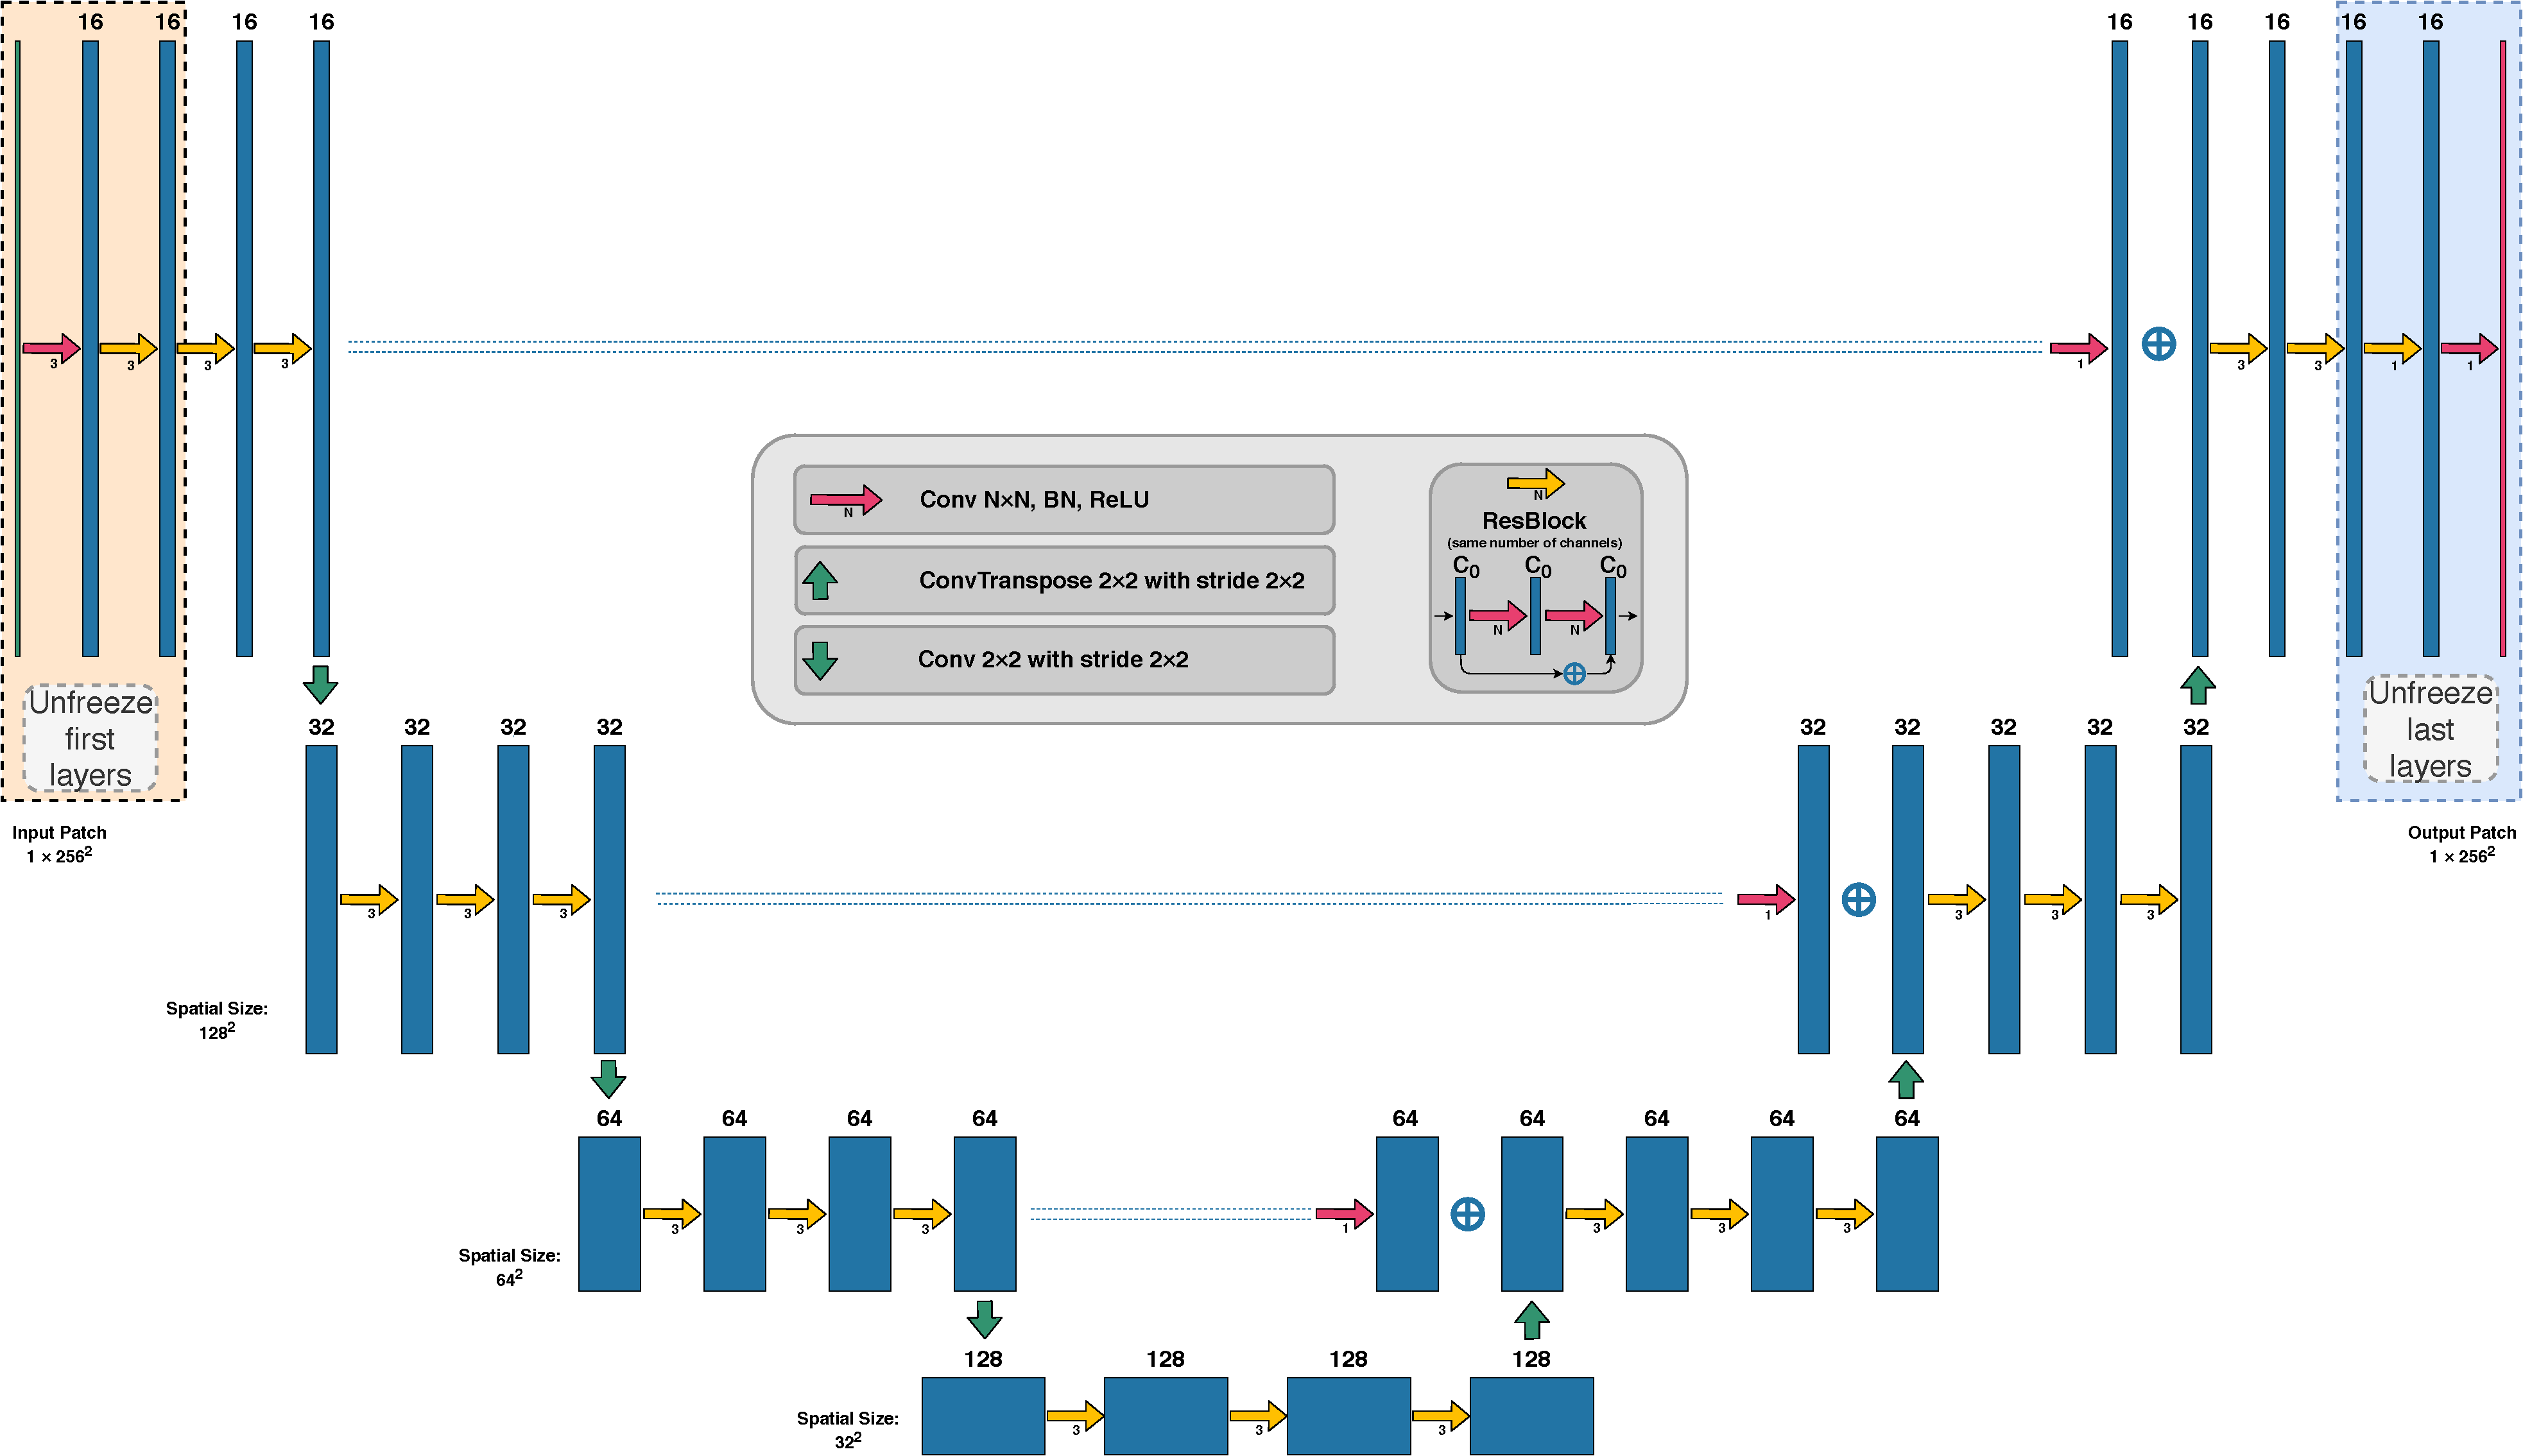
\includegraphics[width=\linewidth]{Dissertation/Figures/2_mri/unet2d_da.pdf}
	\caption{The architecture of 2D U-Net \cite{ronneberger2015u} with minor modification we use in our work. In the scenarios implying network weights freezing, either the first or last three convolutional layers are available for fine-tuning. These layers contain an equal amount of filters (16) of the same size, which means that in both scenarios an approximately equal number of parameters is fine-tuned.}
	\label{fig:mri:unet2d_da}
\end{figure}

Additionally, we introduced minor changes to keep up with the state-of-the-art level of architectures. We use residual blocks \cite{he2016deep} instead of simple convolutions, for this was shown to improve segmentation quality \cite{milletari2016v}. We also apply convolutional layer with $1 \times 1 \times 1$ kernel to the skip-connections. We change the channel-wise concatenation at the end of skip-connections to the channel-wise summation --  it reduces memory consumption and preserves the number of channels in the following residual blocks. We keep it without changes for the rest of the experiments. %To reduce the dependence of the results on the architecture we also carried out the experiments for vanilla U-Net.
%TODO: appendix


\subsection{Adaptive fine-tuning}

Supervised DA in medical image segmentation traditionally relies on explicit decisions regarding which layers of a neural network should be fine-tuned. However, as we discussed above, there is no clear consensus on whether the initial or final layers of the network should be targeted. Moreover, with the increasing complexity of neural network architectures---often involving skip connections and residual pathways---the challenge extends to identifying the ``first'' layers within these intricate structures. Residual networks, for instance, can behave like ensembles of shallower networks \cite{veit2016residual}, complicating the decision-making process regarding which layers to adapt for optimal domain transfer.
%\cite{bakas2018identifying}

To address these challenges, we propose an extension of the SpotTune framework \cite{guo2019spottune} tailored for supervised DA in medical image segmentation, which we call \textbf{SpotTUnet}. SpotTUnet introduces a dynamic and adaptive approach to layer selection, leveraging a policy network to make real-time decisions on whether to fine-tune or freeze specific layers within a network.

\begin{figure}[!h]
	\centering
	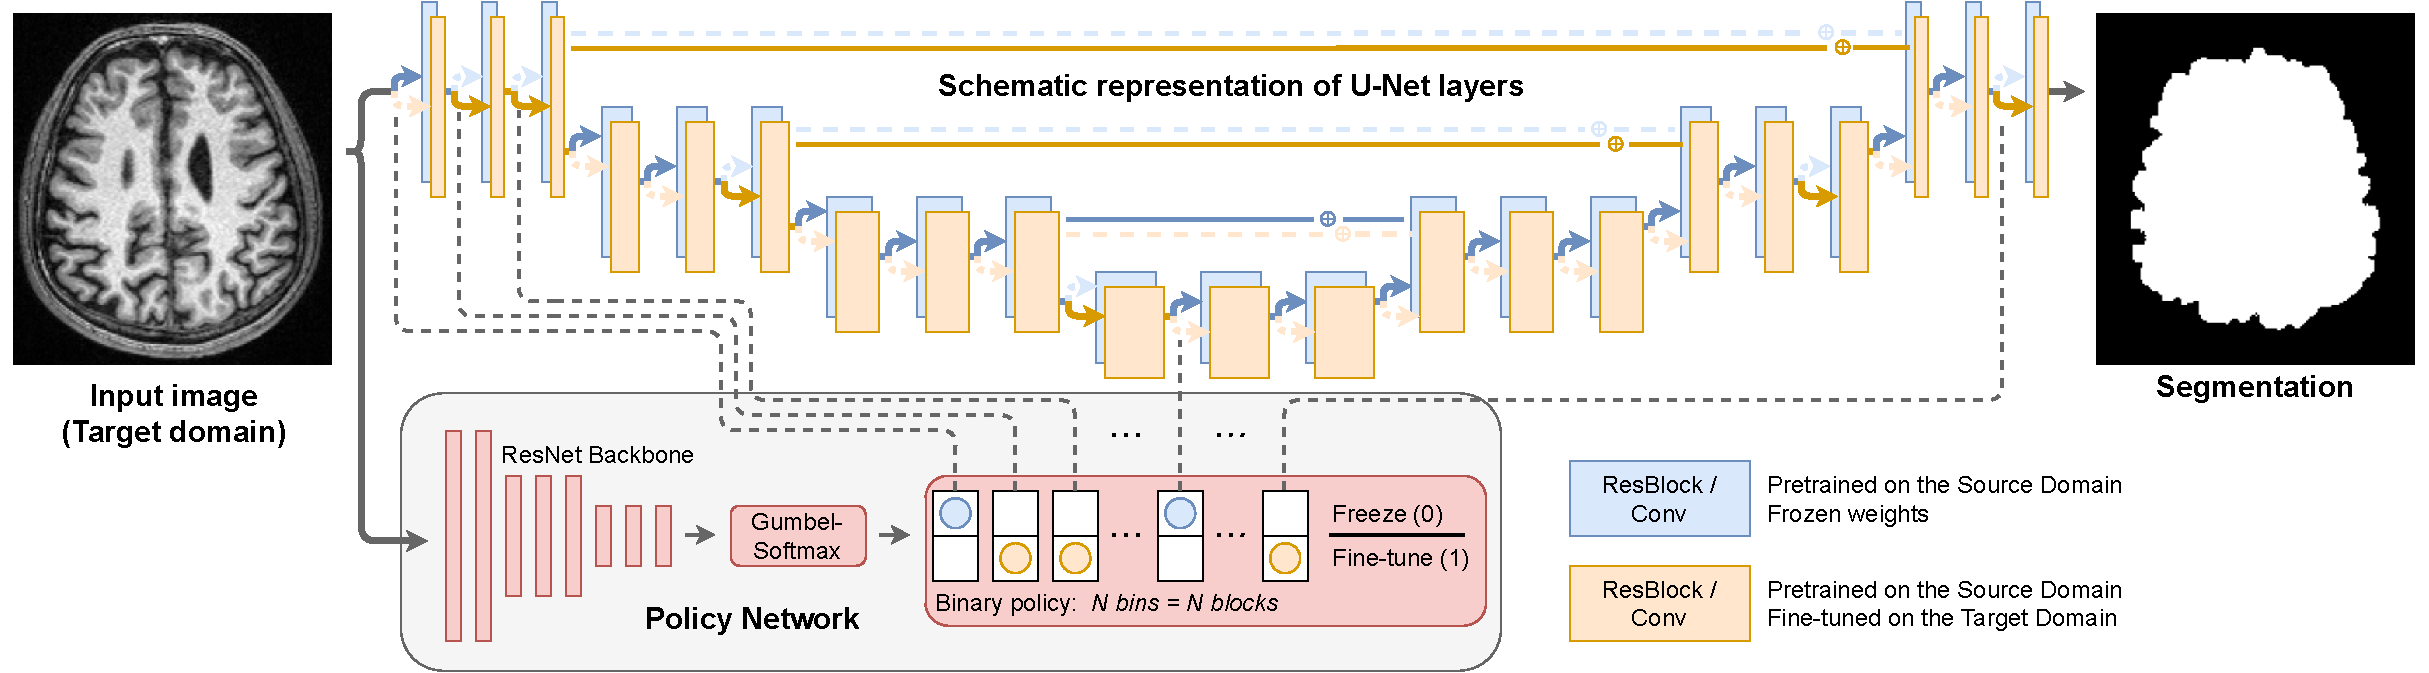
\includegraphics[width=\textwidth]{Dissertation/Figures/2_mri/spottune_seg.pdf}
	\caption{SpotTUnet architecture for the supervised DA in medical image segmentation. The U-Net backbone is pretrained on the source domain. This network is frozen (blue blocks) and has a copy (orange blocks) that is fine-tuned on the target domain. The policy network is simultaneously trained on the target domain to output binary decisions for each pair of blocks from the segmentation networks: use the frozen block (blue) vs. use the fine-tuned block (orange).}
	\label{fig:spottune_seg}
\end{figure}

SpotTUnet consists of three main components: two copies of the main segmentation network and a policy network, as illustrated in Figure~\ref{fig:spottune_seg}. The segmentation  U-Net network, which is described in Section~\ref{sec:mri:method:sft}, is initially pretrained on the source domain dataset. Then, this model is duplicated into two versions and supplemented with the policy network:

\begin{enumerate}
	
	\item \textbf{Frozen Network (Blue Blocks):} The first copy retains the pretrained weights and remains fixed during the fine-tuning process. This network serves as a baseline, preserving the knowledge learned from the source domain.
	
	\item \textbf{Fine-Tuned Network (Orange Blocks):} The second copy is subject to fine-tuning on the target domain dataset. This network adapts to the new domain, with its weights initialized with the pretrained ones and being updated based on the target data.
	
	\item \textbf{Policy Network (Red Blocks):} This model is responsible for predicting whether each block in the segmentation network should use the frozen or fine-tuned version. It outputs a pair of logits for each of the $N$ blocks (block represents a residual block in our case). A softmax function is applied to these logits, converting them into probabilities for a binary classification task:
	\begin{itemize}
		\item Class 0: Use the frozen block from the pretrained network.
		\item Class 1: Use the fine-tuned block from the updated network.
	\end{itemize}
	
\end{enumerate}

The output for the $l$-th block is then computed as:

\begin{equation}
	x_l = I_l ( x ) F_l ( x_{l-1} ) + (1 - I_l ( x )) \tilde{F}_l ( x_{l-1} ),
\end{equation}

\noindent
where $F_l$ and $\tilde{F}_l$ represent the frozen and fine-tuned versions of the $l$-th block, respectively, and $I_l(x)$ is the binary indicator derived from the Policy Network’s prediction.

Policy Network is trained concurrently with the fine-tuning of the segmentation network. During each iteration, Policy Network makes ``soft'' predictions for each block, which we binarize (into $I_l(x)$) to determine whether to use the frozen or fine-tuned block. To ensure gradient flow through the binary decision-making process, we employ the Gumbel-Softmax trick, as proposed in the original SpotTune methodology \cite{guo2019spottune}. This approach allows gradients to be propagated through the binary indicator $I_l(x)$, enabling end-to-end training.
% TODO: expand on gumbel softmax; cite Gumbel-Softmax

In addition to the standard segmentation loss ($\mathcal{L}_{segm}$), we introduce a regularization term to control the number of blocks that are fine-tuned:

\begin{equation}
	\mathcal{L} = \mathcal{L}_{segm} + \lambda \sum_{l=1}^N \left( 1 - I_l (x) \right),
\end{equation}

\noindent
where $\mathcal{L}$ is the resulting loss and $\lambda$ is a regularization parameter that balances the segmentation performance and the number of fine-tuned blocks. The regularization term encourages the model to fine-tune fewer blocks, which is particularly beneficial when only a limited amount of annotated target data is available. %The intuition behind this approach is that fewer fine-tuned blocks reduce the risk of overfitting to the target domain.

While the original SpotTune framework includes a more complex global policy (Global-k), which enforces uniform fine-tuning across all images by constraining them to adapt the same $k$ blocks, we propose a simplified regularization strategy. Our approach introduces an $\mathbb{L}_1$ regularization term that directly minimizes the total number of fine-tuned blocks, leading to a more deterministic and interpretable policy. With only one tunable parameter ($\lambda$), this approach is easier to optimize and more adaptable to different data availability scenarios. A higher $\lambda$ value enforces stronger regularization, leading to fewer fine-tuned blocks, which is especially desirable when the target domain data is limited.

Below we compare SpotTUnet with the other fine-tuning approaches and extensively analyze domain shift anatomy using obtained Policy Network.


\section{Experiments}


\subsection{Data}

We conducted all experiments using the publicly available CC359 dataset \cite{souza2018open}, which consists of 359 head MRI scans. These scans were acquired using scanners from three different vendors: Siemens, Philips, and General Electric. Each vendor's scanners operate at two different magnetic field strengths, 1.5 T and 3 T, resulting in a total of six distinct domains within the dataset. The data distribution is balanced across these domains, with the exception of the Philips 1.5 T domain, which contains only 59 subjects. Using this dataset, we address the brain segmentation task from brain MRI scans.

For preprocessing, we applied two straightforward steps. First, all scans were resampled to a uniform voxel resolution of $1 \times 1 \times 1$ mm using linear interpolation. Second, the voxel intensities of the resampled images were normalized to a range between 0 and 1 before being fed into the network. No additional preprocessing was applied to the data.


\subsection{Evaluation metrics}

The quality in medical image segmentation problems is typically assessed using the Dice Score \cite{bakas2018identifying}, which is defined as:

\begin{equation}
	\label{eq:dice_score}
	\text{Dice Score} = \frac{2 \cdot |A \cap B|}{|A| + |B|},
\end{equation}

\noindent
where $A$ and $B$ represent the predicted and ground truth masks (sets of voxels), respectively. This metric measures the voxel-wise overlap between the two masks, providing a volumetric assessment of segmentation quality. However, in brain segmentation, the accuracy of delineating the brain's edges is a crucial indicator of model performance. Given that edge regions constitute a relatively small portion of the brain's overall volume, the Dice Score may lack sensitivity in capturing the quality of boundary delineation.

To address this limitation, we also employ the \textbf{Surface Dice Score} \cite{nikolov2021clinically}, which specifically evaluates how closely the predicted and ground truth surfaces align. Although the Surface Dice metric shares the same mathematical formula as the Dice Score (Eq. \ref{eq:dice_score}), in this context, $A$ and $B$ correspond to the surfaces of the segmented regions rather than entire volumes. The key difference lies in the concept of \textit{tolerance}, which specifies the maximum allowable distance between corresponding surface voxels for them to be considered as matching.


For our experiments, we report results using a tolerance of 1 mm, as we find this threshold to be sufficiently sensitive to variations in the predictions across different methods.

To further evaluate the effectiveness of each domain adaptation (DA) method, we calculate the proportion of the gap between the Oracle and Baseline scores that the method closes. This proportion, denoted as $D_R$, is defined as follows:

Finally, to assess each DA method for a particular source-target pair we calculate the share of the gap between Oracle and Baseline this method closes. We denote this share $D_R$ and define it the following way:

\begin{equation}
	D_R = \dfrac{D - D_B}{D_O - D_B} = \dfrac{\Delta(transferring)}{\Delta(oracle)},
\end{equation}

\noindent
where $D_O$ represents the Oracle Surface Dice Score on the target domain, $D_B$ is the Baseline score on the target domain, and $D$ is the score of the adaptation method under consideration. This metric provides a clear and interpretable measure of how effectively each DA method improves upon the Baseline, relative to the Oracle. Oracle and Baseline are defined in Section~\ref{sec:mri:exp:setup}.


\subsection{Architecture and Training}

In this study, we opted for a 2D U-Net architecture \cite{ronneberger2015u} rather than a 3D CNN, as it allows us to explore the performance of various approaches on a very limited amount of labeled data from the target domain--specifically, a subset of slices from a single scan. All necessary modifications to the original U-Net architecture are detailed in Section~\ref{sec:mri:method:sft}. Additionally, we conducted baseline experiments using a 3D U-Net \cite{cciccek20163d}, observing a similar decline in segmentation quality. We also repeated the experimental pipeline with the vanilla U-Net to confirm the consistency of our results.

On the source domain, the model was trained for 100 epochs, beginning with a learning rate of $10^{-2}$, which was reduced to $10^{-3}$ at epoch 80. For domain transfer, we fine-tuned the model for 60 epochs, starting with a learning rate of $10^{-3}$ and reducing it to $10^{-4}$ at epoch 45. Each epoch comprised 100 iterations of stochastic gradient descent with Nesterov momentum (set to $0.9$). During each iteration, we randomly sampled a slice, cropped it to a size of $256 \times 256$, and formed a mini-batch of $32$ such samples, which were then passed through the network. Binary Cross-Entropy was used as the segmentation loss function ($\mathcal{L}_{segm}$).

Training for 100 epochs required approximately 4 hours on a 16GB NVIDIA Tesla V100 GPU on Zhores supercomputer \cite{zacharov2019zhores}.


\subsection{Experimental setup}
\label{sec:mri:exp:setup}

We conducted three primary groups of experiments to evaluate our approach. Throughout this section, the term \textit{scan} refers to a complete 3D MRI study, while \textit{slice} denotes a 2D section of a scan.


\subsubsection{Baseline and Oracle}

To assess the suitability of the CC359 dataset for DA experiments, we first established a \textbf{Baseline} for cross-domain model transferability. We trained six separate models, each on a distinct domain, and then tested each model across the remaining target domains. This Baseline provides a foundational comparison for subsequent experiments.

The model's performance within the source domain was evaluated using 3-fold cross-validation, referred to as the \textbf{Oracle} score. This score represents the ``ideal'' reference score for all transfer methods, though it is theoretically possible for some methods to surpass Oracle in certain cases.

In the subsequent transfer experiments, models trained on the entire source domain were transferred to target domains. We evaluated the effectiveness of these methods by calculating the fraction of the performance gap between the oracle and the baseline that each method was able to close. This metric provides a clear and interpretable measure of methods performance.


\subsubsection{Predefined fine-tuning}

The first focus of our study is on three supervised domain adaptation strategies: fine-tuning the entire model (\textbf{all layers}), fine-tuning only the \textbf{initial layers}, and fine-tuning only the \textbf{final layers}.

Our goal was to assess the performance of these strategies under varying conditions of data availability, particularly in scenarios with an extreme scarcity of target domain data. Preliminary experiments indicated that segmentation quality begins to decline when fewer than five scans are available, which aligns with findings from previous studies \cite{valverde2019one}, where segmentation performance decreased as the number of voxels in the ground truth mask was reduced. By using a 2D network, we were able to work with a subset of slices from a single scan instead of reducing the ground truth mask, which was not feasible for our task.

We varied the amount of available data, starting with 3 and 1 target MRI scans. Leveraging our 2D architecture, we further subsampled slices from a single scan at fractions of $1/2$, $1/3$, $1/6$, $1/12$, $1/24$, and $1/36$. In these scenarios, slices were evenly sampled with a consistent step; for example, in the $1/3$ scenario, slices 0, 3, 6, and so forth were selected. The total numbers of slices available for fine-tuning are 800, 270, 135, 90, 45, 24, 12, 8, respectively.

We repeat these experiments for each of the 30 source-target pairs in the CC359 dataset.


\subsubsection{Adaptive fine-tuning}

Again, the six domains in the dataset yielded $30$ source-target pairs, leading to $30$ supervised DA experiments. Since we needed to select SpotTUnet hyperparameters, we reserved one source domain (Siemens, $1.5$ T) and its corresponding 5 source-target pairs for SpotTUnet validation, using the remaining 25 pairs to test designed DA approaches.

For the $5$ validation pairs, we first tuned the temperature parameter of Gumbel-Softmax ($\tau$) through grid-search, exploring values $\tau \in \{ .01, .1 , .5, 1, 2, 5 \}$. The number of annotated slices from the target domain was fixed at 270 (equivalent to one scan). Next, we optimized the $\lambda$ parameter for each level of target data availability via grid-search over $\lambda \in \{0, 1, 3 , 5, 7, 10, 12, 15, 20 \} \times 10^{-3}$. The latter validation experiment and all testing experiments addressed the same scenarios for target data scarcity, with $8$, $12$, $24$, $45$, $90$, $270$, and $800$ slices available for fine-tuning. The optimal $\lambda$ value was fixed for each data scarcity scenario and applied to SpotTUnet during testing on the remaining $25$ pairs.

%\textbf{Discussion of the additional setups.} Despite the authors of \cite{isensee2018no} suggest focusing on the pipeline rather than the peculiarities of an architecture, we support our claim with the same line of experiments with vanilla U-Net architecture \cite{ronneberger2015u}. Moreover, extremely limited amounts of data available raise the question of augmentation, thus we repeat all the experiments for both architectures, introducing simple augmentation techniques: rotations and symmetric flips. We place all the results for vanilla U-Net and the results for the original net trained with augmentation in Supplementary Materials while discussing them in Sec. \ref{sec:results}.

%In our preliminary experiments we also tried other supervised DA setups. First, instead of fine-tuning, we trained the model from scratch on joint data from the source and the target domains. Secondly, we trained the model from scratch on data from the target domain only. We do not include aforementioned strategies in the further analysis for they yield extremely poor results.


\section{Results}


\subsection{Baseline and Oracle}

Table~\ref{tab:mri_baseline} illustrates the domain shift problem in our experiments. When evaluating the 2D U-Net model on the source domain using cross-validation, we observe high Surface Dice values, representing the \textit{Oracle} performance (diagonal elements). However, when the model is transferred to a different domain without fine-tuning (non-diagonal elements, referred to as the \textit{Baseline}), there is a significant drop in segmentation quality. The best scores are highlighted in bold, while the lowest are indicated in italics to emphasize the impact of domain shift.




\begin{table}[h!]
	\centering
	\caption{\textbf{Cross-domain model performance without fine-tuning.} Column headers represent the source domains on which the model was trained, while row headers correspond to the target domains on which the model was tested. ``Sm,'' ``GE,'' and ``Ph'' refer to vendors Siemens, GE, and Philips, respectively. Results are reported as Surface Dice Scores, with corresponding standard deviations in parentheses.}
	\label{tab:mri_baseline}
	
	\begin{tabular}{lcccccc}
		\toprule
		& Sm, 1.5T & Sm, 3T & GE, 1.5T & GE, 3T & Ph, 1.5T & Ph, 3T \\
		\midrule
		Sm, 1.5T & \textbf{.85 (.12)} & .51 (.15) & .72 (.08) & .56 (.13) & .71 (.10) & .71 (.07) \\
		
		Sm, 3T   & .72 (.08) & \textbf{.88 (.03)} & .70 (.07) & .67 (.10) & .63 (.10) & .66 (.06) \\
		
		GE, 1.5T & .39 (.14) & \textit{.09 (.05)} & \textbf{.87 (.05)} & \textit{.30 (.10)} & .55 (.19) & .48 (.08) \\
		
		GE, 3T   & .80 (.05) & .63 (.13) & .66 (.10) & \textbf{.89 (.03)} & .67 (.10) & .67 (.06) \\
		
		Ph, 1.5T & .63 (.08) & \textit{.25 (.07)} & \textbf{.87 (.03)} & .43 (.06) & \textbf{.89 (.03)} & .46 (.08) \\
		
		Ph, 3T   & .54 (.13) & .34 (.13) & .70 (.11) & .37 (.10) & .47 (.14) &  \textbf{.86 (.04)} \\
		\bottomrule
	\end{tabular}
\end{table}



\subsection{Predefined fine-tuning}

In this section, we compare three approaches to supervised DA: fine-tuning the entire model (\textit{all layers}), fine-tuning only the \textit{initial (first) layers}, and fine-tuning only the \textit{final (last) layers}.

We analyze how the relative improvement score $D_R$ depends on the amount of training data available from the target domain. Figure~\ref{fig:gap} shows the average scores across 30 possible source-target domain pairs. The figure also presents the distribution densities of these scores for each strategy.

\begin{figure}[h!]
	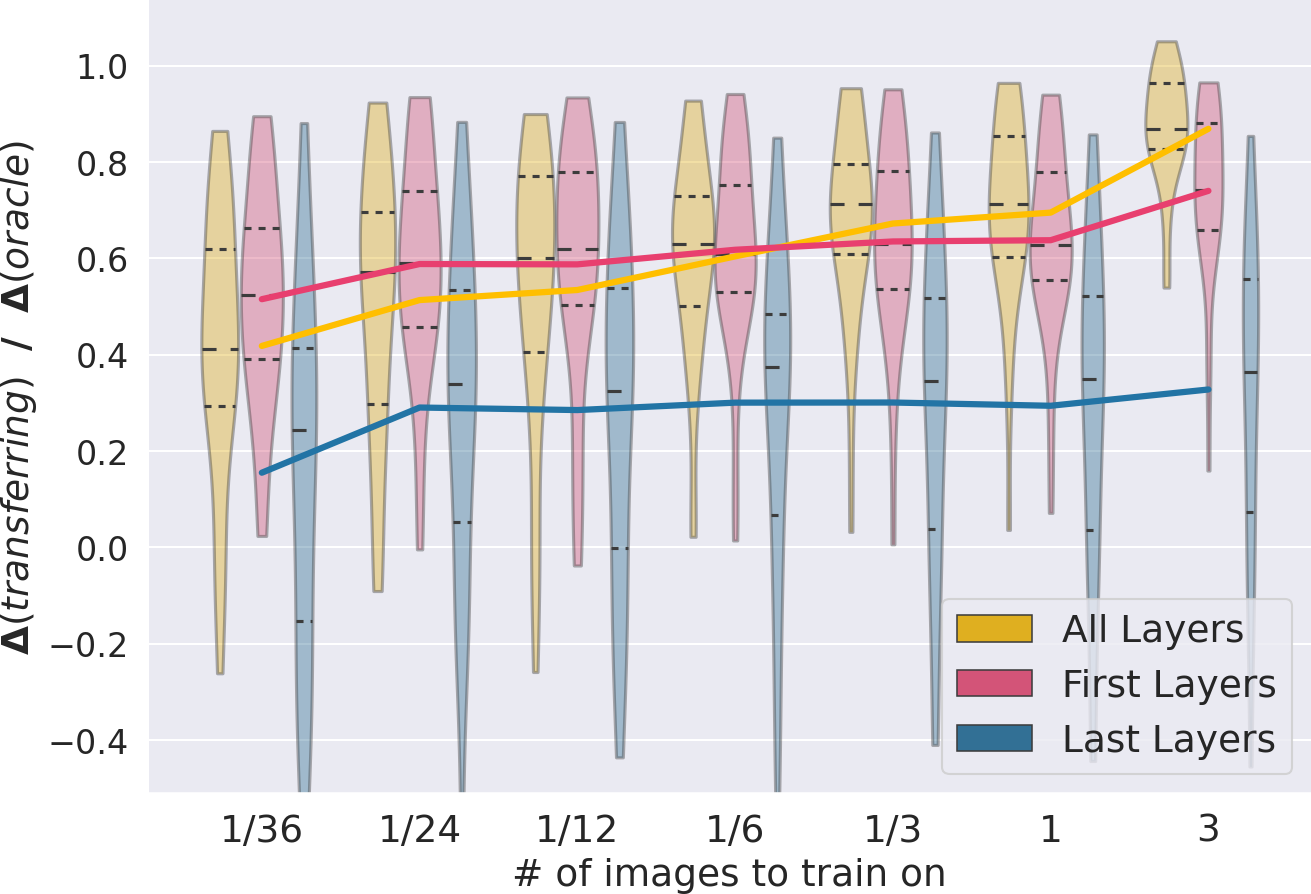
\includegraphics[width=\linewidth]{Dissertation/Figures/2_mri/gap.png}
	\caption{Dependence of the relative Surface Dice improvement (y-axis, $D_R$) on the availability of target domain data (x-axis) for the three transfer strategies. The lines represent average scores, while the density distributions reflect scores across 30 source-target pairs for each strategy.}
	\label{fig:gap}
\end{figure}

In Figure~\ref{fig:winners}, we report the number of source-target pairs where a given method outperforms the others (summing to 30 across all methods for each setup). Contrary to common assumptions, our results show that fine-tuning the initial layers significantly outperforms fine-tuning the final layers in our task. This finding suggests that low-level features, which correspond to the image's intensity profile, can be more effectively re-learned than high-level features, which are associated with different brain structures and distinct shapes.

Moreover, under conditions of extreme data scarcity, fine-tuning the initial layers proves to be more advantageous than fine-tuning the entire model. This makes the former approach particularly valuable in practical scenarios where annotated target domain data is limited.

\begin{figure}[h]
	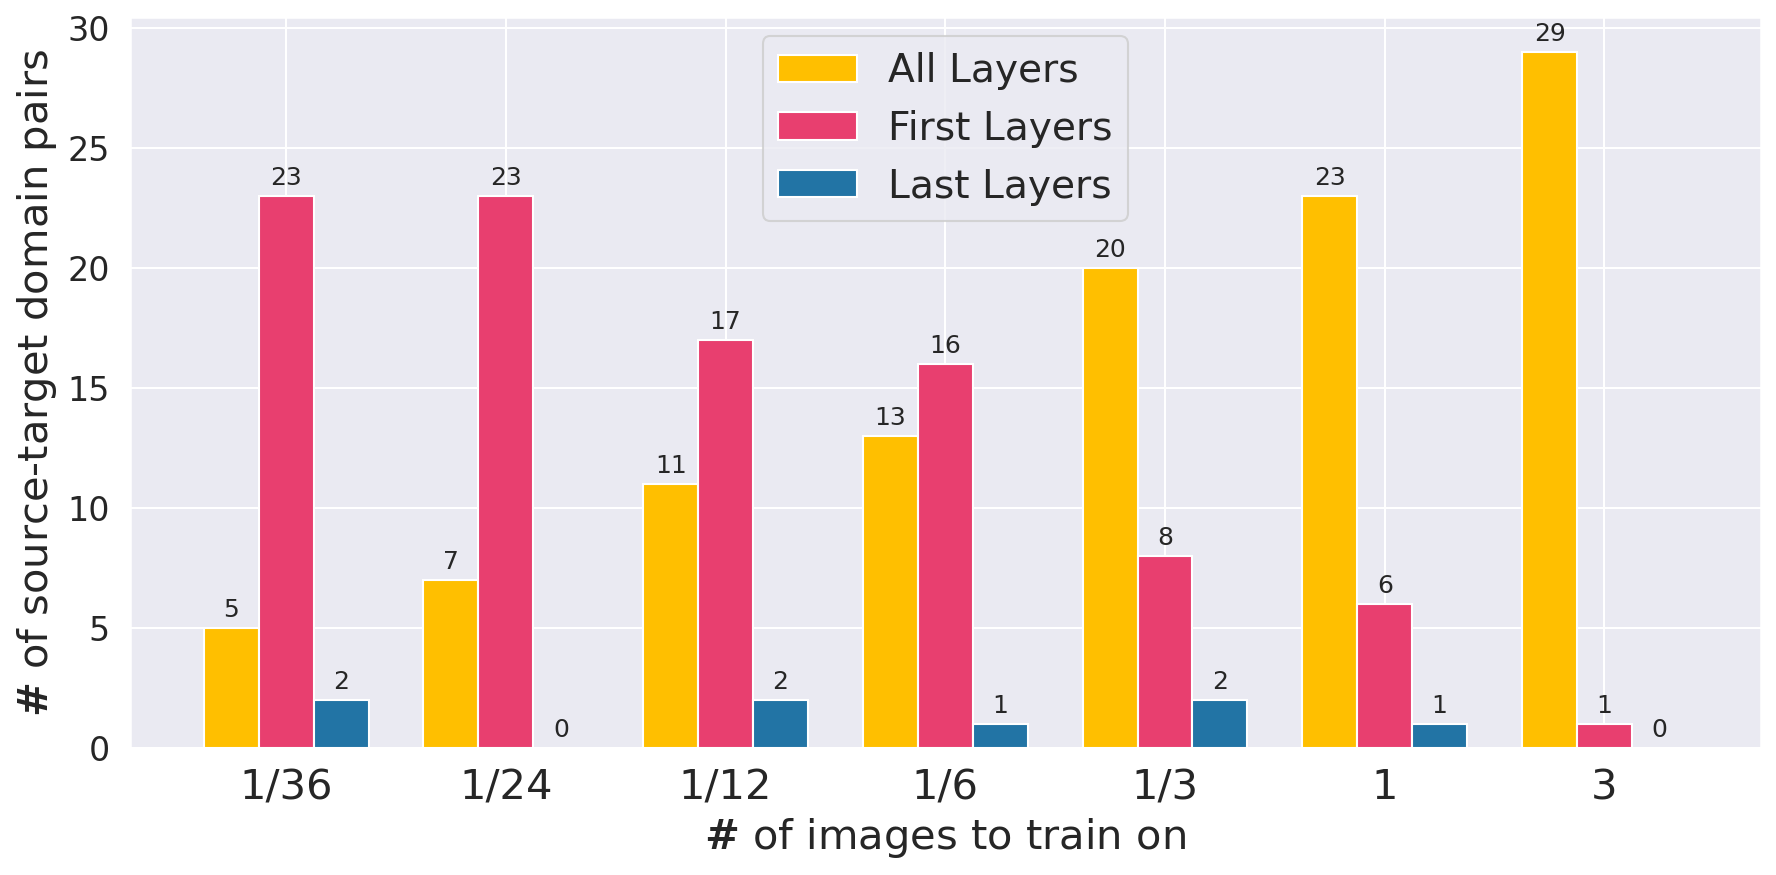
\includegraphics[width=\linewidth]{Dissertation/Figures/2_mri/winners_1.png}
	\caption{Effectiveness of each domain adaptation strategy based on target domain data availability. Each bar represents the number of source-target pairs for which a given method is the most effective.}
	\label{fig:winners}
\end{figure}

The observed trends remain consistent even when substituting U-Net with residual blocks with the vanilla U-Net or adding augmentation. %\todo{Results for these setups are available in the Supplementary materials.}% TODO: add supplementary results to Appendix


\subsection{Adaptive fine-tuning}

We begin by tuning and selecting the hyperparameters for SpotTUnet through validation.

The temperature of the Gumbel-Softmax is set to $\tau = 0.1$, while the optimal regularization parameter $\lambda$ is determined separately for each data scarcity scenario; see Figure~\ref{fig:lambda}. It is important to note that the stability of Gumbel-Softmax training is highly sensitive to the choice of $\tau$, so we recommend validating different values of $\tau$ early in the deployment of SpotTune-like architectures.

We found that a positive regularization term significantly benefits most data scarcity setups: the surface Dice Score with the optimal $\lambda$ is significantly higher ($p < 10^{-3}$, one-sided Wilcoxon signed-rank test) than that of the corresponding model without regularization. The only exception is the case with 800 available target slices (approximately three 3D images), where the optimal $\lambda$ is close to zero, and increasing $\lambda$ leads to a drop in quality; see Figure~\ref{fig:lambda}. This suggests that while SpotTUnet can learn the optimal policy without regularization when target data is abundant, regularization significantly enhances DA performance when target data is scarce.

\begin{figure}[h!]
	\centering
	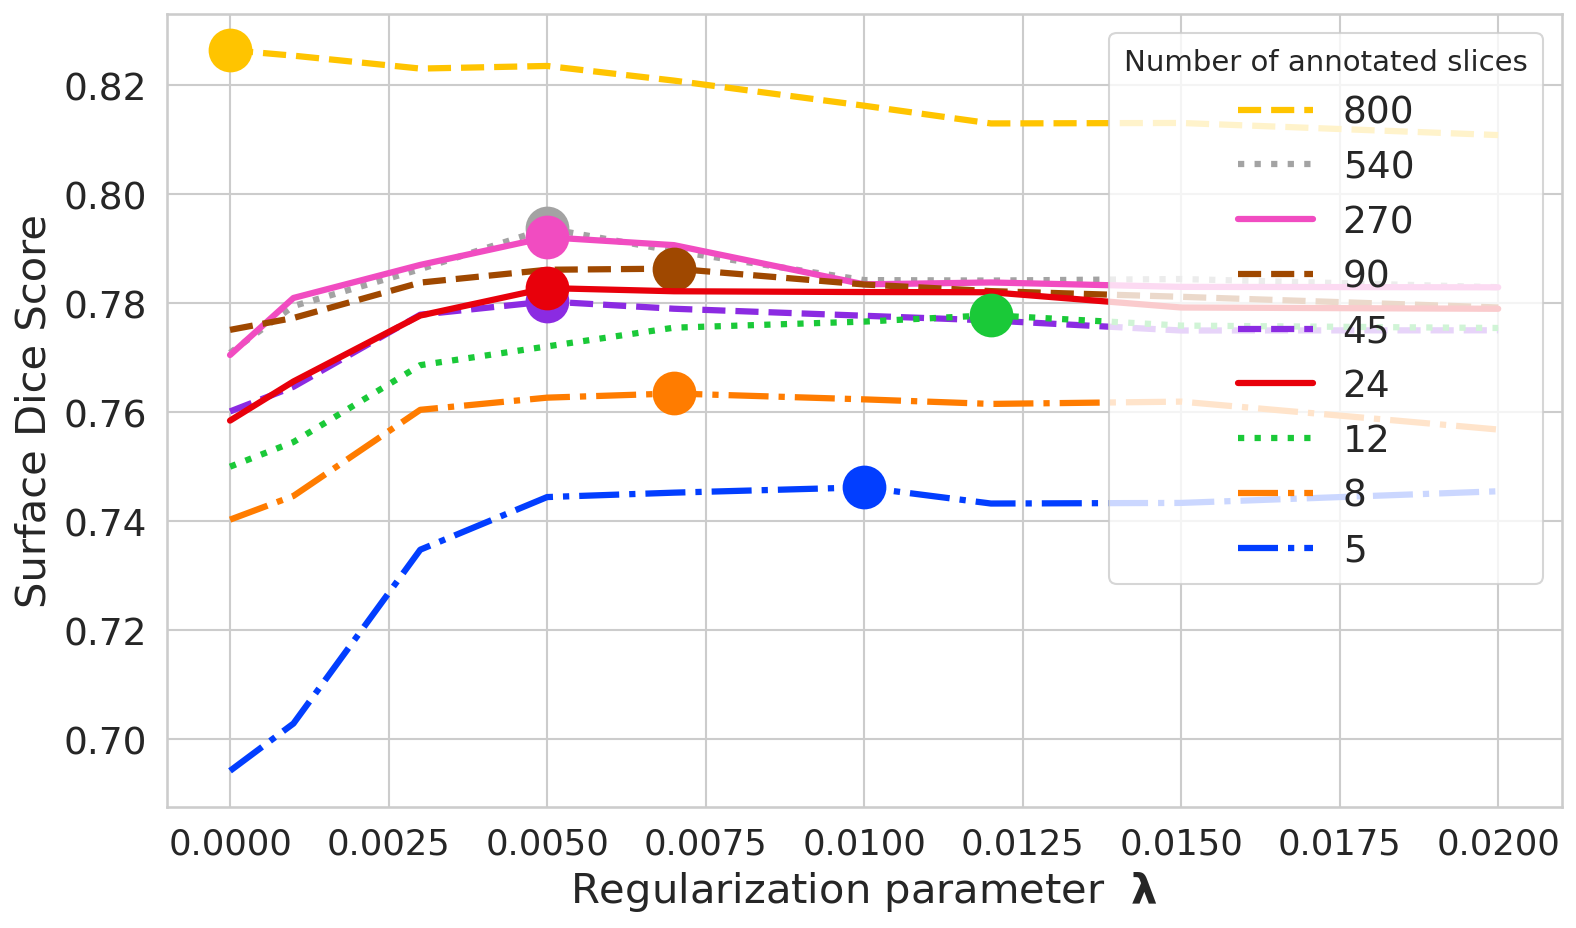
\includegraphics[width=\textwidth]{Dissertation/Figures/2_mri/k_reg.png}
	\caption{Validation performance of SpotTUnet as a function of the regularization parameter $\lambda$. Each point represents the average Surface Dice Score across 5 validation experiments. Each line corresponds to a different amount of annotated data from the target domain, with bold points indicating the optimal $\lambda$ values in terms of Surface Dice Score.}
	\label{fig:lambda}
\end{figure}

% and \textit{histogram matching}
%Histogram matching achieves an average surface Dice Score of only 0.29, which is even lower than the baseline average of 0.55, so we exclude both methods from further comparison in Figure~\ref{fig:sdcs}.
Next, we compare SpotTUnet with the previously developed approaches: \textit{Fine-Tune All Layers} and \textit{Fine-Tune First Layers}. Strategy of \textit{fine-tuning the last layers} is excluded from comparison due to previously shown poor performance. Figure~\ref{fig:sdcs} shows the distributions of the surface Dice Scores (violin plots) alongside their average values (lines). Our results demonstrate that SpotTune performs on par with the best of the other methods, regardless of the severity of target data scarcity.

\begin{figure}[h!]
	\centering
	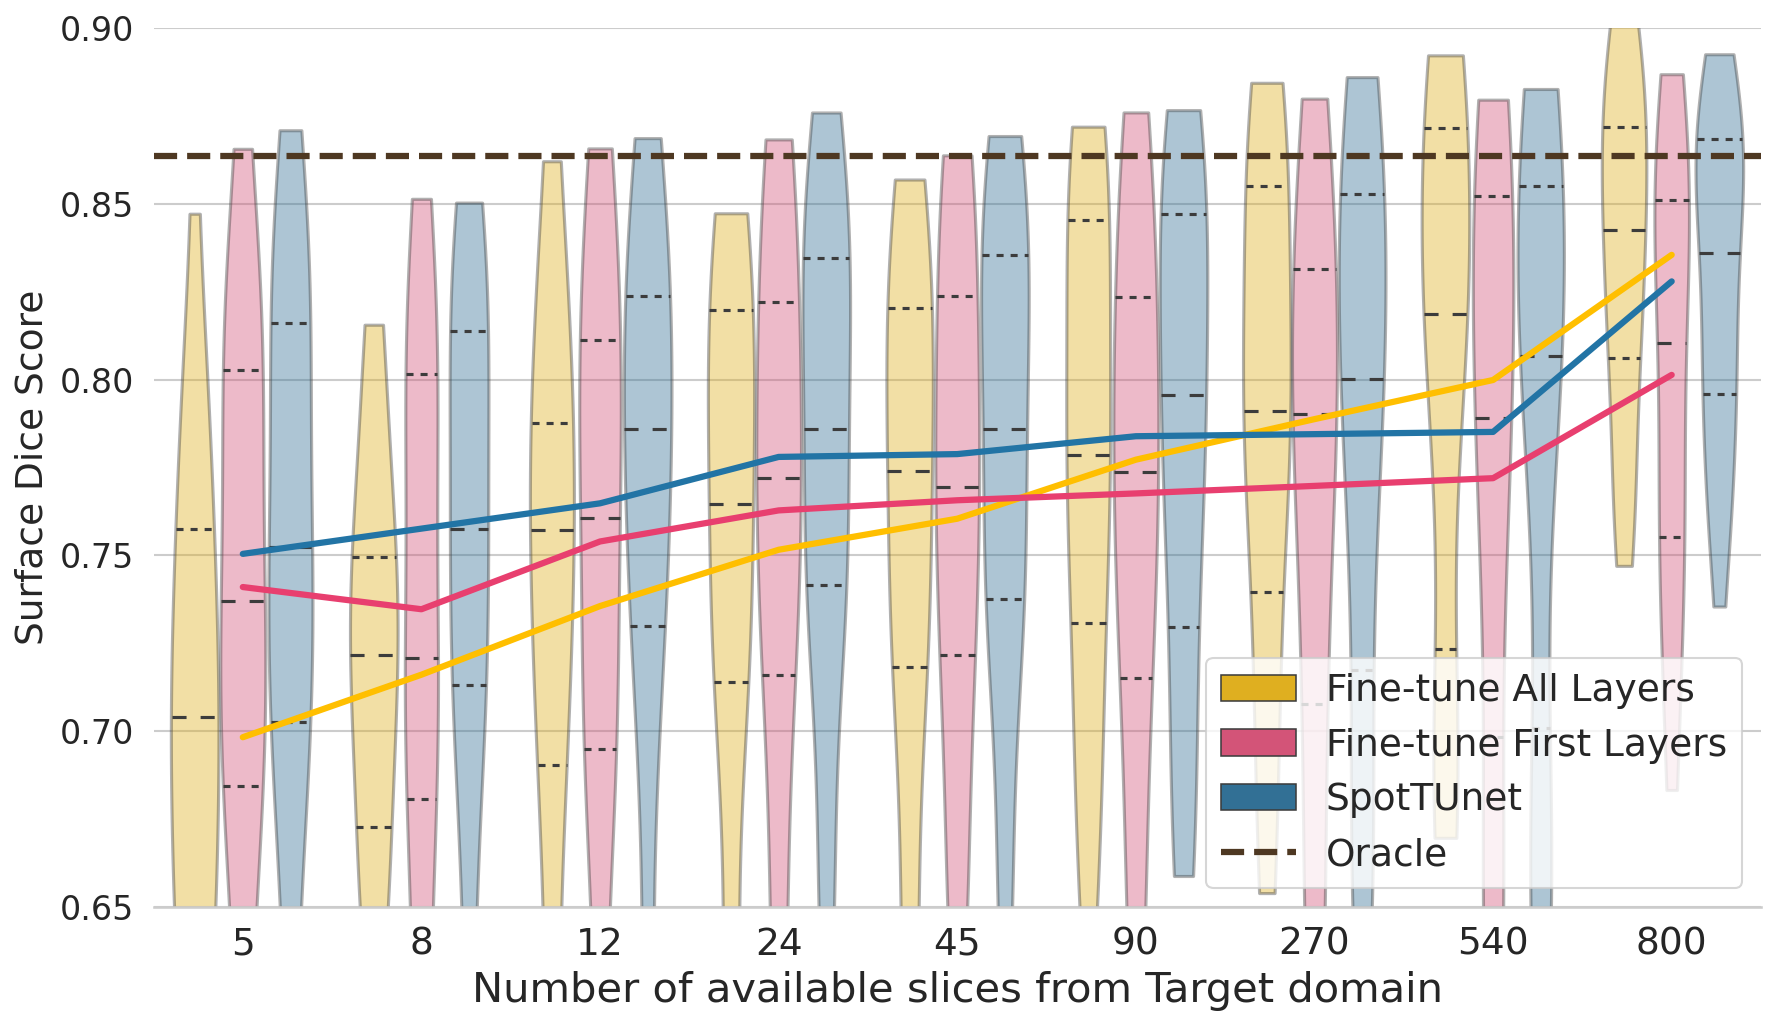
\includegraphics[width=\textwidth]{Dissertation/Figures/2_mri/sdsc.png}
	\caption{Performance of different methods as a function of target domain data availability.}
	\label{fig:sdcs}
\end{figure}

Finally, we examine the policy learned by SpotTUnet on the test data by calculating the frequency with which each layer is fine-tuned versus kept pretrained and frozen. The layer-wise visualization is shown in Figure~\ref{fig:layerswise_template}. We find that blocks in the encoder part of the U-Net are more frequently fine-tuned, particularly when annotated data is scarce. However, these are not necessarily the first layers (e.g., those preserving the original resolution), which contrasts with our previous findings, reported in \cite{shirokikh2020first}. We hypothesize that the SpotTUnet policy highlights layers that should be fine-tuned for optimal performance. Consequently, feature maps preceding these frequently fine-tuned layers might be more susceptible to domain shifts. It may be worthwhile to explore whether unsupervised DA approaches \cite{kamnitsas2017unsupervised, zhao2021robust} could benefit from passing these domain-shift-prone feature maps to adversarial networks---a hypothesis we leave for future research.

\begin{figure}[h!]
	\centering
	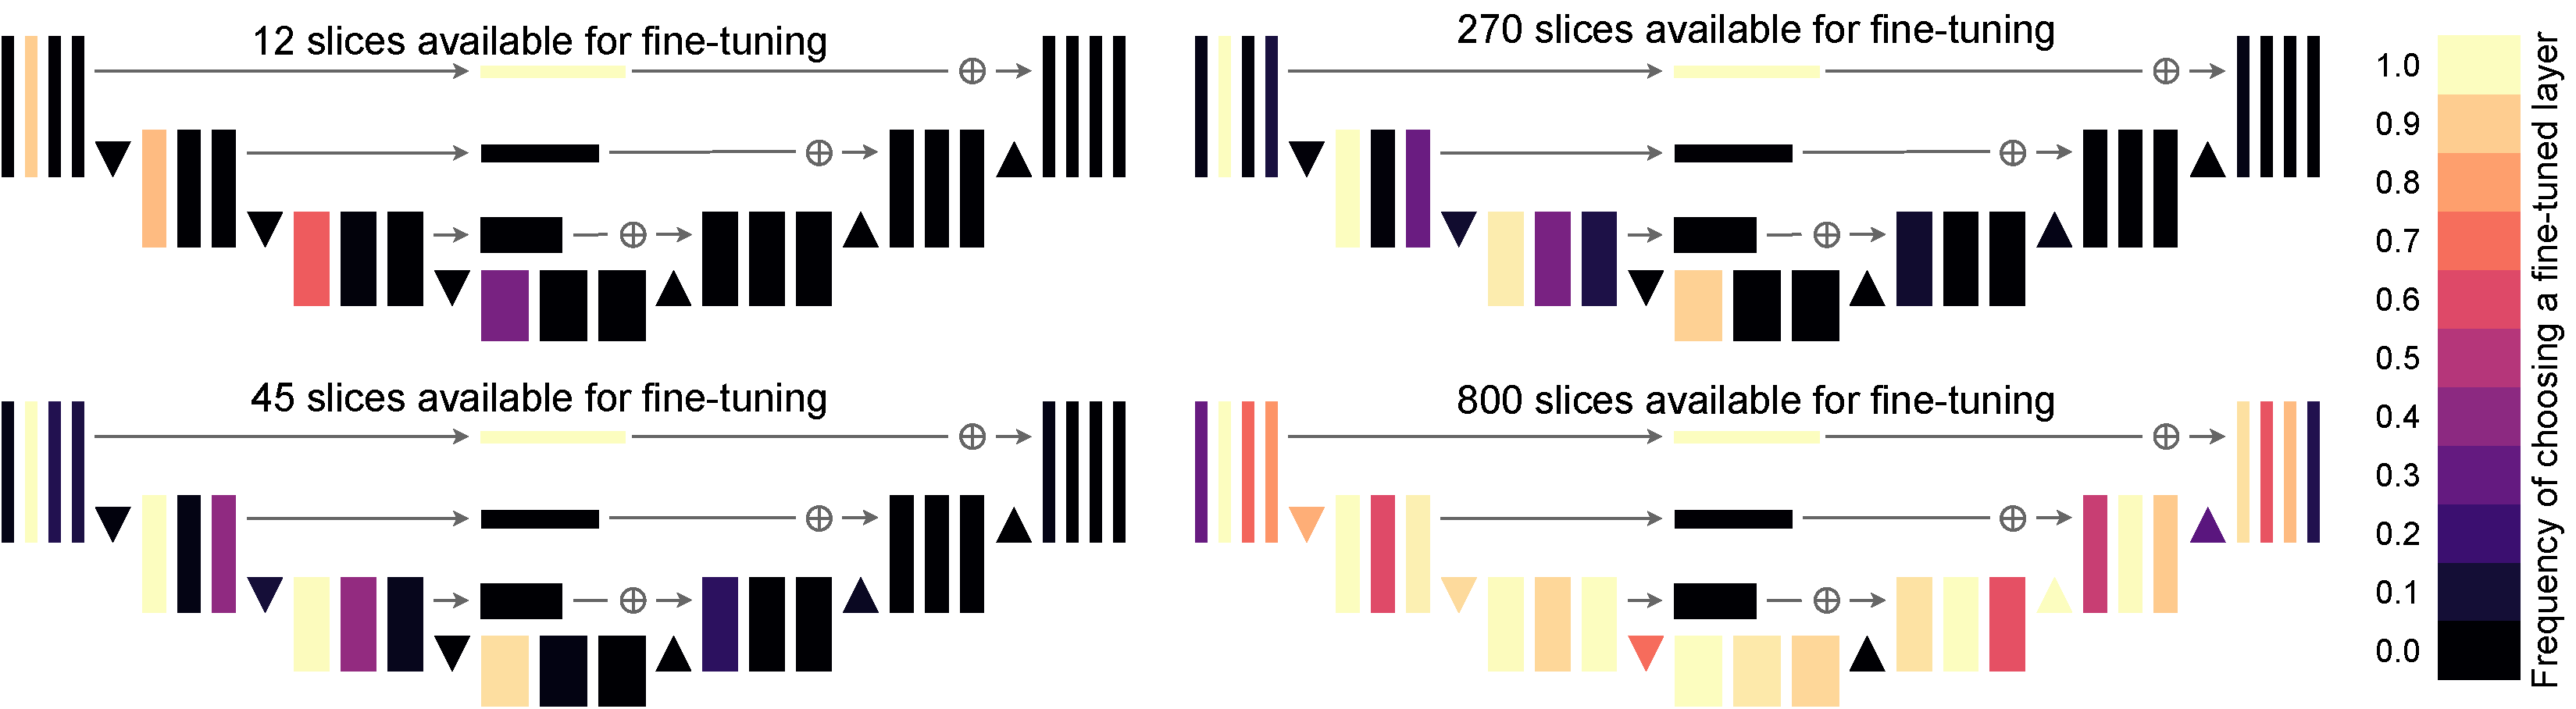
\includegraphics[width=\textwidth]{Dissertation/Figures/2_mri/layerwise_template.pdf}
	\caption{Visualization of SpotTUnet's learned policy for different amounts of available target slices: 12 (upper-left), 45 (bottom-left), 270 (upper-right), and 800 (bottom-right). Colored blocks correspond to residual blocks, with triangular blocks indicating convolutions that perform $\times 2$ up- or down-sampling.}
	\label{fig:layerswise_template}
\end{figure}

The differences between the policies observed here and those reported in the original SpotTune paper \cite{guo2019spottune} (where mostly final layers were fine-tuned) can be attributed to the fundamental differences between Transfer Learning (TL) and DA. In TL, the data often varies significantly in nature, so fine-tuning the later layers is necessary. In DA, however, the datasets are semantically similar (e.g., brain MRI scans), meaning that domain shifts are primarily low-level, requiring fine-tuning of the earlier layers.


\section{Summary}

This study highlights a significant drop in segmentation quality when naively transferring models between the domains of the CC359 dataset. We hypothesize that the low-level feature maps in this dataset are more susceptible to domain shifts than those from deeper layers, making the initial layers a primary source of performance degradation. Our findings support this hypothesis, demonstrating that fine-tuning the initial layers yields better results than fine-tuning the final layers. Moreover, in scenarios with limited annotated data in the target domain, fine-tuning the initial layers proves to be more effective than fine-tuning the entire network.

We also introduce a new approach for supervised domain adaptation in medical image segmentation, called SpotTUnet. Our experiments show that SpotTUnet maintains the quality of previous methods while eliminating the need to switch between different approaches based on the availability of target data. Additionally, SpotTUnet autonomously learns which layers to fine-tune for optimal performance in the target domain, offering a valuable policy that identifies the network layers most affected by domain shifts. We believe this policy could guide the development of more robust unsupervised domain adaptation methods by specifically targeting the initial or SpotTUnet-identified layers.


